\chapter{Secure Hierarchical In-network data aggregation} % (fold)
\label{cha:Secure Hierarchical In-network data aggregation}

We describe the Secure Hierarchical In-network data aggregation $\textit{(SHIA)}$ protocol of \cite{chan2006secure} as our work enhances this protocol by making it more efficient and adding new capabilities to the protocol. The goal of $\textit{SHIA}$ is to compute aggregate functions (such as $\textit{SUM}$, $\textit{AVERAGE}$, $\textit{COUNT}$) of the sensed values by the sensor nodes while assuming that a portion of the sensor nodes are controlled by an adversary which is attempting to skew the final result.

\section{Network Assumptions}
\section{Security Infrastructure}
\section{Attacker Model}
\section{Problem Definition}
\section{The SUM Aggregate Algorithm}
	In this algorithm, the aggregate function $f$\ is summation meaning that we want to compute $a_{1} + a_{2} + \dotsc + a_{n}$, where $a_{i}$\ is the sensed data value of the node $i$.
	This algorithm has three main phases:
	\begin{itemize}
		\item Query dissemination
		\item Aggregate commit
		\item Result checking
	\end{itemize}

	\section{Query dissemination}
		Prior to this phase an aggregation trees is created using a tree generation algorithm.
		We can use any tree generation algorithm as this protocol works on any aggregation tree structure.
		For completeness of this protocol, one can use Tiny Aggregation Service (TaG)\cite{madden2002tag}.
		TaG uses broadcast message from the base station to initiate a tree generation.
		Each node selects its parent from whichever node it first receives the tree formation message.
		One possible aggregation tree for given network graph in Figure \ref{fig:ng} is shown in Figure \ref{fig:at}. 
		\begin{figure}[hp]
			\centering
			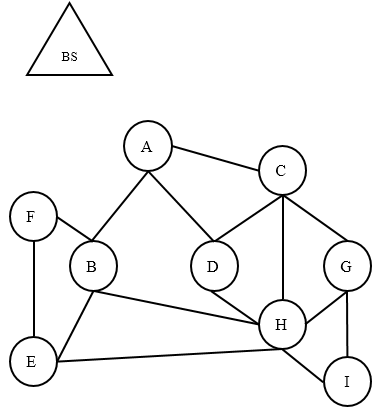
\includegraphics[scale = 1]{images/network-graph.png}\\
			\caption{Network graph}
			\label{fig:ng}
		\end{figure}
		
		To initiate the query dissemination phase, the base station broadcasts the query request message with the query nonce $N$\ in the aggregation tree. 
		The query request message contains new query nonce $N$\ for each query to prevent replay attacks in the network.
		It is very important that the same nonce is never re-used by the base station.
		$SHIA$\ uses \textbf{hash chain} to generate new nonce for each query. 
		A hash chain is constructed by repeatedly evaluating a pre-image resistant hash function $h$\ on some initial random value, the final value (or ``anchor value'') is preloaded on the nodes in the network.
		The base station uses the pre-image of the last used  value as the nonce for the next broadcast.
		For example, if the last known value of the hash chain is $h^m(R)$, then the next broadcast uses $h^{m-1}(R)$ as the nonce; $R$ is the initial random value.  
		A hash chain prevents an adversary from predicting the query nonce for future queries as it has to reverse the hash chain computation to get an acceptable pre-image.

		\begin{figure}[hp]
			\centering
			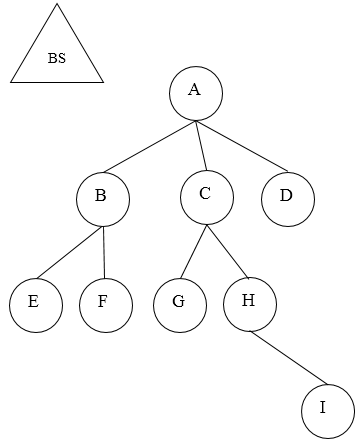
\includegraphics[scale = 1]{images/aggregation-tree.png}\\
			\caption{Aggregation tree for network graph in Figure \ref{fig:ng}}
			\label{fig:at}
		\end{figure}		

	\section{Aggregate commit} 
	% (fold)
		\label{sub:aggregate_commit}
		The aggregation-commit phase constructs cryptographic commitments to the data values and to the intermediate in-network aggregation operations.
		These commitments are then passed on to the base station by the root of an aggregation tree.
		The base station then rebroadcasts the commitments to the sensor network using an authenticated broadcast so that the rest of the sensor nodes in the network can verify that their respective data values have been incorporated into the final aggregate value.

		\subsection{Aggregate commit: Naive Approach}
		% (fold)
			\label{sub:aggregate_commit_naive_approach}
			In the naive approach, during aggregation process each sensor node computes a cryptographic hash of all its inputs (including its own data value).
			The aggregation result along with the hash value called a label, is then passed on to the parent in the aggregation tree.
			The label is defined in Definition \ref.
			Figure \ref{fig:naive-commitment-tree} shows a commitment tree.
			Conceptually, a commitment tree is a hash tree defined in \cite{przydatek2003sia} with additional aggregate information attached to the nodes to help us in result checking phase.
			\begin{figure}[hp]
				\centering
				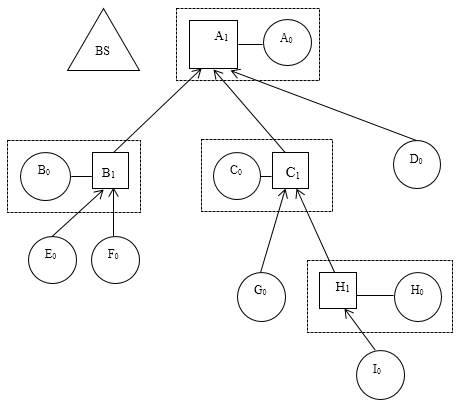
\includegraphics[scale = 1]{images/naive-commitment-tree.png}\\
				\caption{Naive commitment tree}
				\label{fig:naive-commitment-tree}
			\end{figure}

			\begin{definition}
				Definition 3 A commitment tree is a tree where each vertex has an associated label representing the data that is passed on to its parent. The labels have the following format:
				count, value, complement, commitment Where count is the number of leaf vertices in the subtree rooted at this vertex; value is the SUM aggregate computed over all the leaves in the subtree; complement is the aggregate over the COMPLEMENT of the data values; and commitment is a cryptographic
				commitment.
				\label{def:label}
			\end{definition}
		% subsection aggregate_commit_naive_approach (end)

	% section aggregate_commit (end)

Then elaborate your approach.
Two differences:
	data-item format
	CT generation being root in as many trees as possible